\documentclass{standalone}

\usepackage{tikzbricks}

\usepackage{tikz-3dplot}

\begin{document}


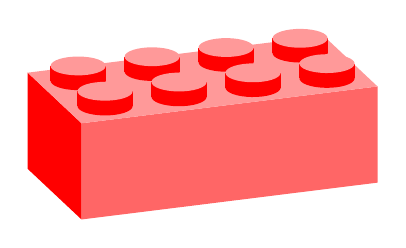
\begin{tikzpicture}
\brick{4}{2}
\end{tikzpicture}


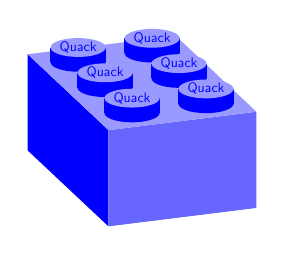
\begin{tikzpicture}
\brick[color=blue,studtext={Quack}]{2}{3}
\end{tikzpicture}


\begin{tikzpicture}
\brick[color=orange]{1}{1}
\end{tikzpicture}

\tdplotsetmaincoords{70}{110}
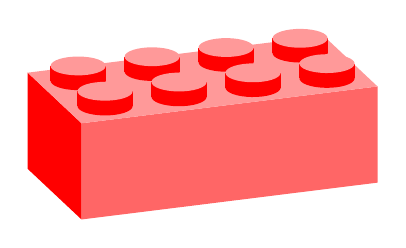
\begin{tikzpicture}
\brick{4}{2}
\end{tikzpicture}


\begin{tikzpicture}
\brick[color=teal,scale=2]{1}{1}
\end{tikzpicture}

\tdplotsetmaincoords{70}{160}
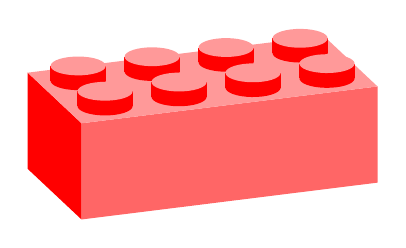
\begin{tikzpicture}
\brick{4}{2}
\end{tikzpicture}

\tdplotsetmaincoords{70}{180}
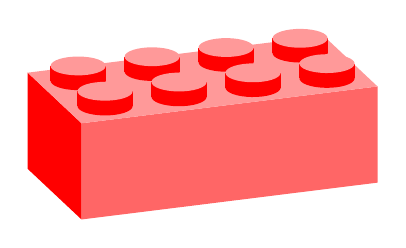
\begin{tikzpicture}
\brick{4}{2}
\end{tikzpicture}

\begin{wall}
  \wallbrick[color=teal]{3}{1}
  \wallbrick[color=red]{1}{1}
  \addtocounter{brickx}{2}
  \wallbrick[color=orange]{1}{1}
  \newrow
  \wallbrick[color=blue]{1}{1}
  \wallbrick[color=cyan]{6}{1}
\end{wall}




\end{document}